% !TeX root = ../thesis_main.tex

\section{Prototype Implementation}\label{sec::solution_code}
This section describes the implementation of the DevContainer concept in a real project that is currently developed by the Symbic GmbH. At the beginning, the initial state of the project is described as well as the goal to be achieved, then the concept from section \ref{sec::solution_concept} is applied and an architecture for the DevContainer setup is designed. The following section describes the implementation process and puts special emphasis on potential errors and which catches there are to minimize them. Finally, the end state is compared to the previously set goal.

    \subsection{Project Information and expected Target State}
    % Name for the project
    The project presented here is currently developed and maintained by Symbic GmbH. It is a system for deploying and managing \ac{IoT} devices from the agricultural sector and is based on a microservice architecture. The \ac{IoT} devices are used on agricultural machinery to assists vehicle operators in his work by providing an interface between the lead vehicle and trailed machinery. Vehicle and harvest information can be displayed and the position of the vehicle is tracked. With the system presented here, new interfaces can be installed on the devices and existing ones can be adapted, while also providing a web interface to display the collected device data. Various \ac{API}s provide different functionalities, which are made available by multiple microservices. In order for the system to operate, various auxiliary services are required, including \ac{SSH}-servers and MQTT-brokers. For the brevity and clarity of this paper, only a subsection of the system is presented in this thesis. This makes a further, more realistic implementation possible without going into an excessive description of the system which would have a detrimental effect on the concept of DevContainers. A detailed description of the project is given in the following section. \newline
    The goal is to test the concept described in section \ref{sec::solution_concept} for applicability in a real project, any encountered challenges are described below and possible solutions to them are given as well. In the end the resulting solution is compared to the initial expectations described in section \ref{sssec::goal}.

        \subsubsection{About the Project}\label{ssec::project}
        % !TeX root = ../thesis_main.tex
\begin{figure}[]
    \centering
    \tikzstyle{block} = [rectangle, draw, fill=green!80!blue!70,
    text width=5em, text centered, rounded corners, minimum height=4em]
    \tikzstyle{line} = [draw, very thick, color=black!50, -latex']

    \begin{tikzpicture}[
        align=center,
        scale=0.2,
        node distance=3.5cm,
        auto]

        % Frontend
        \node [] (user) {
\includegraphics[width=.08\textwidth]{fig/user.png}\\User};
        \node [block, left of=user, xshift=-15mm] (webapp) {
\includegraphics[width=.5\textwidth]{fig/vue.png}\\WebApp};

        % Microservice Cluster
        \node [block, below of=webapp, xshift=-20mm, yshift=-5mm] (authbackend) {
\includegraphics[width=.4\textwidth]{fig/php.png}\\Auth-Backend};
        \node [block, below of=webapp, xshift=20mm, yshift=-5mm] (deviceapi) {
\includegraphics[width=.7\textwidth]{fig/node1.png}\\System-API};
        \node[draw,dashed,fit=(authbackend) (deviceapi), label={[above]MS\\Cluster}] (microcluster) {};

        % MQTT Service
        \node [block, right of=deviceapi, xshift=2mm] (mqttcon) {
\includegraphics[width=.7\textwidth]{fig/node1.png}\\MQTT Connector};
        \node [block, right of=mqttcon, xshift=7mm] (mqttbroker) {
\includegraphics[width=.3\textwidth]{fig/mqtt-logo-small.png}\\MQTT Broker};
        \node[draw,dashed,fit=(mqttbroker) (mqttcon), label={[above]MQTT\\Service}] (mqttservice){};

        % DB Stuff
        \node[database,label=below:SQL\\User \acs{DB},database radius=.8cm,database segment height=0.42cm, below of=authbackend] (userdb) {};
        \node[database,label=below:Logs\\Mongo\acs{DB} ,database radius=.8cm,database segment height=0.42cm, below of=webapp, yshift=-38mm] (logdb) {};
        \node[database,label=below:SQL\\Device \acs{DB},database radius=.8cm,database segment height=0.42cm, below of=deviceapi] (devicedb) {};

        % Device
        \node [below of=mqttbroker] (device) {
\includegraphics[width=.1\textwidth]{fig/device.png}\\Devices};

        % Edges & Paths
        \path [line] (user) -- node [text width=2.5cm, align=center, above]{Interacts\\with} (webapp);
        % To APIs
        \path [line] (webapp) -- node [text width=3.5cm, align=center, left, yshift=3mm, xshift=4mm]{Validates Authentication} (authbackend);
        \path [line] (webapp) -- node [text width=4cm, align=center, right, yshift=3mm]{Provides Device Data \& Functionality } (deviceapi);
        % To DB
        \path [line] (authbackend) -- node [text width=2cm, align=center, left, yshift=-2mm]{Connects to} (userdb);
        \path [line] (authbackend) -- node [text width=1cm, above,xshift=10mm, yshift=-5.5mm]{Event Logs} (logdb);
        \path [line] (deviceapi) -- node [text width=1cm, above, xshift=-3.5mm, yshift=-1mm]{} (logdb);
        \path [line] (deviceapi) -- node [text width=2cm, align=center, right, yshift=-2mm]{Connects to} (devicedb);
        % MQTT Device
        \path [line ] (microcluster) -- node [align=center, above] {Uses} (mqttservice);
        \path [line ] (mqttcon) -- node [text width=2cm, align=center, above] {\acs{REST} API for} (mqttbroker);
        \path [line,transform canvas={xshift=2mm}] (device) -- node [text width=2.5cm, align=center, right]{} (mqttbroker);
        \path [line, transform canvas={xshift=-2mm}] (mqttbroker) -- node [text width=3cm, align=center, left, yshift=-3mm]{Subscribe\\\& Publish\\Messages} (device);

    \end{tikzpicture}
    \caption{IoT Web Service Architecture}\label{fig::arch}
\end{figure}


        % % !TeX root = ../thesis_main.tex
% \subsection{Figure Alternatives}
\begin{figure}[!h]
    \centering
    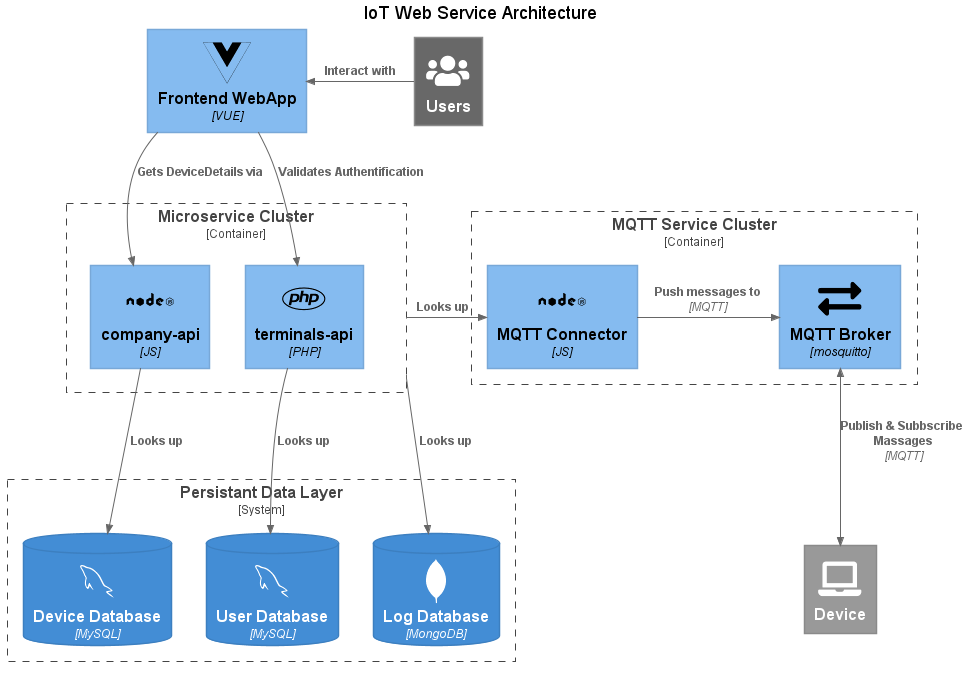
\includegraphics[width=.95\textwidth]{CCI-System-clean.png}
    \caption{IoT Web Service Architecture - [Alternative]}\label{fig::arch}
\end{figure} % Alternative
        \noindent As described above, the project builds on a microservice architecture. The advantage of this architecture is that it allows the use of different technologies for individual applications. Communication between applications takes place via a platform-independent protocol. If the load on a part of the application becomes critical, new instances of this application can be created with little effort and added to the service-stack.\newline
        Figure~\ref{fig::arch} visualizes the architectural structure of the entire service. Each green box refers to a standalone application and contains an icon with the technology used. Users of this service only directly interact via the web interface (WebApp). The web interface is created with the \ac{JS} framework \wordhighlight{Vue.js}, which generates a static bundle of HTML, CSS and \ac{JS} files, served by a static web-server. In order to access the system, users must authenticate themselves in the WebApp. This is done via the authentication backend (Auth-Backend), written in PHP. In addition to the authentication, this application also performs additional tasks, which will be neglected, for reasons of brevity. Provided the user is authenticated, the WebApp can display internal information and functions of all deployed \ac{IoT} devices. These dynamic information are provided by the NodeJS-based System-\ac{API}. All \ac{API} endpoints are implemented under the compliance with the \ac{OAS}. The \ac{OAS} allows easy discoverability and understanding of the \ac{API} for humans and computers. It also provides versioning support of \ac{API}s to avoid unexpected errors in other applications. These applications are part of the microservice cluster, delimited by the dashed frame, which is actively being developed by Symbic; in addition to the services listed here, the cluster consists of more services.\newline
        Both, the Auth-Backend and the System-\ac{API}, have their own SQL databases that persistently stores relevant information. However, both applications write user events to a shared event database. MongoDB is used to provide an schema flexible NoSQL database. In order to send specific instructions to, or receive information from a \ac{IoT} device, the system \ac{API} communicates with an MQTT-broker via the NodeJS-based MQTT-Connector. The MQTT-Connector provides an unified \ac{REST} \ac{API} for publishing and subscribing messages over the MQTT protocol. On a larger scale, the MQTT-Connector is consumed by several applications and is therefore a standalone application. Since only a part of this project is considered here, the System-\ac{API} is the only application communicating with the MQTT-Connector. In addition to the MQTT-broker, other auxiliary services such as SSH servers are used, which are not discussed here for reasons of brevity. The MQTT-broker exposes a public endpoint offering various topics which devices can subscribe or publish to. Via this system the user can trigger a command in the web interface, which is then processed and logged by the system \ac{API}. Sequentially it is made available on the MQTT-broker via the MQTT-Connector. \ac{IoT} devices, that have subscribed to the corresponding topic, receive this command and execute it. The result is then published to another topic and can be accessed in the same way via the WebApp. Since the \ac{IoT} devices are connected to the Internet via SIM cards, and are therefore on a restricted mobile carrier network, they are not directly accessible from the Internet. Through the described system, the \ac{IoT} devices can execute commands from the outside without being accessible via the Internet.

        \subsubsection{Initial State of the Projects Development Environment}
        New developers joining the project have to clone all four repositories, install NodeJS 14, a specific version of the \ac{XAMPP} stack and must customize its configuration. Furthermore, the PHP project requires the package manager \wordhighlight{composer}, which must be installed separately. The configuration details must be taken from the documentation or are provided by a collaborator. In order to test the whole, unified system, developers also need to install a MQTT-broker and the MongoDB database. Both applications need an initial administrator user, which needs to be created beforehand, and the corresponding credentials need to be accessible by each \ac{API}, which is made possible through the creation of an \code{.env} file - a file, which is not tracked in the \ac{VCS}. Then, a database and its schema needs to be created. Eventually network ports have to be adjusted and secrets for signing tokens have to be created.
        Thus, to set up a new environment, developers must install the all required frameworks, set up databases, customize ports, and enter connection information in the applications \code{.env} file. These steps are necessary to get the project running properly, whereas the setup of developer tools like debugger has not been considered yet. Even in a small project, this can take some time, especially if one is not yet familiar with the project.\newline
        Still, even experienced project members encounter challenges when working on such a project. Before the APIs can be launched, it must be ensured that the databases and other auxiliary tools are already running. To start all four applications (WebApp, Auth-backend, System-API, MQTT-Connector) a developer needs four terminal sessions or a terminal multiplexer to operate all applications. The program's outputs (logs) are distributed over all four sessions and can neither be linked to each other directly, nor are they filterable, nor searchable. When everything is running, developers can contribute value to the project. The restrictions mentioned above do not generally hinder developers in their work unless an error occurs. A merge containing dependency or database schema updates conducted by a team member can cause the environment of others to break, resulting in a hard to debug error due to the lack of uniformity. The lack of consistent, reproducible setups is the cause for lasting troubleshooting sessions and the well-known iconic saying \textit{"But it works on my machine"}. This mirrors the problems of heterogeneous systems mentioned in section \ref{sec::problem}. It does not matter whether the individual development environments differ form each other or the development environment differs to the production environment. The sheer fact that there are always differences is the main cause of before-mentioned problems. \newline
        These selected problems emerged in just one project. When working on multiple projects, the problem scope increases accordingly. Different databases, runtimes and dependencies further contribute to a greater potential for issues. The lack of project isolation may result in unintended side effects between projects that slow down the development process. To prevent these unnecessary slowdowns, the initial setup of an environment and its operation must be as homogeneous as possible.

        \subsubsection{Goal for the Target State}\label{sssec::goal}
        The goal is that, by using DevContainers, a faster deployment of the project environments is archived, which is uniform among all developers and has greater similarity to the productive environment. This is made possible by the principle of virtualization, which provides a similar environment, regardless of the host. Accordingly, this should avoid system-dependent errors and eliminate the lack of reproducibility. Thus, any system can be used as host operating system, as long as it is supported by Docker. The DevContainer environment to be created is not intended to forcibly replace existing environments, but to provide an alternative solution that is also platform independent. New team members can quickly set up a working environment based on either Windows, Linux or macOS host, while offering an alternative for developers with existing environments, which they can switch to gradually. Thus, a hybrid environment of the traditional development environments and DevContainer should be possible. Developers should also remain free in their choice of editors and utilities.\newline
        At any time, developers should be able to exercise control over the container runtime and the processes within the container. Thus, in the event of an error, they are independently able to replace a non-functioning container with a new one. The DevContainer environment should run locally and not require an Internet connection to external servers or services in order to be unaffected by Internet connection errors. To ease the transition to a DevContainer-based development environment, it must be possible to set up the environment with a single command, as well as to start all services with one command. Developers should not need to have explicit knowledge of how DevContainers work in order to use them.

    \subsection{Applying the DevContainer Approach}\label{ssec::apply}
    This section will apply the concept of DevContainer as described in section \ref{sec::solution_concept} to the Symbic project. First, the rough procedure of the process will be described, followed by the exact implementation and step-by-step descriptions. Problems, possible solutions and limitations of the concept will be described at the end.

        \subsubsection{Approach on the Project}\label{ssec::imp_approach}
        Regarding the goal of a fully comprehensive development environment for all microservices of the Symbic project, each service, each service will get its own DevContainer, as is intended in a microservice architecture. This allows granular control over the individual services and makes it possible to implement a hybrid operation of conventional running services and DevContainers. For this purpose, a \code{Dockerfile.dev} file, which contains all the necessary runtime environments and other developer tools in a pre-built image, must be created for each service. The source code is not copied into the container, but later included via bind-mounts. This prevents a sudden or accidental loss of changes when switching between different editors on the host. Images have to be built less often and can be shared between applications with the same runtime. The orchestration of the individual services is then done with the Docker-Compose tool. Both, the configuration settings of all services, defined in a \code{docker-compose.yml} file, and their Dockerfiles are then stored in \ac{VCS}m according to the \ac{IaC} principle. With the help of the remote extension for \ac{VSCode}, developers can attach themselves to any container process and take full control over the system and the running application.\newline
        Windows is used as the starting point for the development of the setup, as this is the most widely-used operating system for development at Symbic. After the Docker images have been created and tested, they will later be automatically built by the GitLab \ac{CI}. Once the setup is operational on Windows systems, it is tested on other operating systems, and adapted if necessary. Finally, scripts will be provided for the initial download of all repositories and for the database initialization.

        \subsubsection{The Implementation Process}\label{ssec::imp_process}
        The next paragraphs will provide a step-by-step description of the DevContainer architecture's design, starting with the Dockerfiles for the images, over the creation of the \code{docker-compose.yml} file, up to the usage of the environment via \ac{VSCode}.
        \myparagraph{Creating the Dockerfiles}
        The microservices project described in section \ref{ssec::project} is based on two technology stacks. The WebApp, the System-\ac{API} and the MQTT-Connector are all based on the NodeJS runtime, whereas the authentication backend is written in PHP. Accordingly, two variants of Docker images are needed. As already described in section \ref{sssec::docker}, Docker images are created from Dockerfiles. Each statement in a Dockerfile creates a new layer, which allows to build upon of already existing images.\newline
        As a basis for the NodeJS DevContainer the official \code{node:16-bullseye} image is used as a starting. This Debian-based images was chosen because it used in the production environment, come from a trusted source and is updated regularly. Subsequently, it serves as the appropriate basis for the installation of additional tools, such as git, a ssh server, build tools, and the terminal-based editors vim and emacs. As already stated, the source code is not written into the image, because it is mounted into the container via bind-mount at runtime. The complete Dockerfile for the WebApp, the System-\ac{API} and the MQTT-Connector can be found in Listing \ref{code::docker_dev_node}. The installation script used in the Dockerfile make some from Microsoft recommended, low level adjustments to the system and can be found in the appendix.\newline
        % !TeX root = ../thesis_main.tex

\begin{lstlisting}[language=docker, frame=single, caption={NodeJS DevContainer Dockerfile},label=code::docker_dev_node]
# Node.js version: 16-bullseye, 14-bullseye, 12-bullseye
ARG VARIANT=16-bullseye
FROM node:${VARIANT}

# Install needed packages, yarn, nvm and other tools
COPY install-scripts/*.sh /tmp/install-scripts/
RUN apt-get update && bash /tmp/install-scripts/install.sh \
&& apt-get -y install python3 make vim emacs git ssh \
    && npm install -g eslint
\end{lstlisting}

        % % !TeX root = ../thesis_main.tex

\begin{lstlisting}[language=docker, frame=single, caption={NodeJS DevContainer Dockerfile},label=code::docker_dev_node]
ARG NODE_VARIANT="14-buster"
FROM mcr.microsoft.com/vscode/devcontainers/javascript-node:
    ${NODE_VARIANT}

RUN apt-get update && apt-get install -y \
    git zsh ssh python3 make vim emacs
\end{lstlisting}

        However, as for the PHP application, the Dockerfile is more complex, since besides the PHP runtime several plugins are needed that build C/C++ libraries which are not installed by default. After its installation, the \wordhighlight{Apache \acs{HTTP} Server} must be configured accordingly to be able to use these plugins. The official PHP Docker image is again used as a starting point. It is especially built for PHP applications and already contains the Apache-\acs{HTTP}-Server and a package manager for installing PHP extensions. Line 2 in Listing \ref{code::docker_dev_php} specifies the PHP version used, followed by the installation of several development tools. Subsequently, the PHP extensions used for the app and their dependencies are installed. Since this application also provides static assets, this time, the source code is copied into the image, followed by the installation of additional PHP packages with the help of the \wordhighlight{PHP-Composer}. In the last step, the Apache \acs{HTTP} Server is configured and file permissions are adjusted. The image contains all needed resources in order to start the application and also includes several development tools such as the preconfigured \wordhighlight{Xdebug} debugger.\newline
        For both, the NodeJS image and the PHP image, the versions are passed to the Dockerfile as arguments. This makes it possible to influence the version of the used runtime when executing the build process. Thus, multiple images can be built from one Dockerfile without the need to adapt it and developers have the possibility to adapt new runtimes without much effort. During the process of creation, the images were created locally; whereas in productive use, the GitLab \ac{CI} is responsible for creating regularly updated images. The job for creating the images is described in more detail at the end of this section. The images presented here are very extensive in order to offer the developers the greatest possible comfort. DevContainers also work with much narrower images that can be adapted to the needs of the developers over time.

        \myparagraph{Orchestrating the Microservices}
        The applications from the Symbic project illustrated in Figure \ref{fig::arch} need auxiliary services. As a precondition ensuring its full working order, the project requires an SQL-Database, a MongoDB-Server and a MQTT-Broker. By choosing a MySQL-Server, the Eclipse-Mosquitto-Broker and the official MongoDB-Server, free pre-built, official Docker images are available for all these applications. Listing \ref{code::compose_helper} shows how these services are configured in a \code{docker-compose.yml} file in order to be usable for other applications. Each application is defined as a service, containing their corresponding Docker image as an attribute. In order to make the applications usable outside the virtual docker network, the internal network ports are exposed on the host system (see line 7, 16, 22 in Listing \ref{code::compose_helper}). To ensure that the data stored in the container is not lost when it is renewed, volumes are used to store application data persistently on the host. For this purpose, the name of the volume followed by the mount point of the volume in the container is specified in the services volumes property. Typical for Docker, the initial credentials are configured by means of environment variables. In contrast, the Mosquitto-Server is configured by bind-mounting configuration files from the \code{manage-reop/config} folder to \code{mosquitto/config}. Eventually, the respective application ports are exposed on the host.\newline
        % !TeX root = ../thesis_main.tex

\begin{lstlisting}[language=docker-compose-2,caption={Auxiliary Services docker-compose.yml},breaklines=true,label={code::compose_helper}]
version: "3"
services:
  db:
    image: mysql
    environment:
      - MYSQL_ROOT_PASSWORD=yes
    ports:
      - 3306:3306
    volumes:
      - db_sql_data:/var/lib/mysql

  mongo:
    image: mongo:4.4-focal
    environment:
      - MONGO_INITDB_ROOT_USERNAME=root
      - MONGO_INITDB_ROOT_PASSWORD=none
      - MONGO_INITDB_DATABASE=dm-cu-local
    ports:
      - 27017:27017
    volumes:
      - db_mongo_data:/data/db

  mosquitto:
    image: eclipse-mosquitto
    ports:
      - 1883:1883
    volumes:
        - mosquitto_data:/mosquitto/data
        - ./manage-reop/config:/mosquitto/config
\end{lstlisting}

        Without applying the concept of actual DevContainers, the configuration in Listing \ref{code::compose_helper} already enriches the developer experience. Developers do not have to install and configure extra programs, such as databases, but can make them available quickly, uniformly and platform-independently with one command.\newline
        In order to use DevContainers, the individual applications must also be defined as services. Listing \ref{code::compose_service} demonstrates this as an example for the System-\ac{API}: the name of the DevContainer image is used as a starting point, just like in the previous section \ref{sec::solution_concept}. Subsequently, the credentials for the auxiliary services are made available to the application via environment variables. Since the source code is not included in the image, it is mapped by a bind-mount into the container. Now, all the necessary requirements for starting the application in the DevContainer are fulfilled.\newline
        Since the project is a NodeJS application, all dependencies are stored locally in the project directory under the \code{node\_modules} folder. These dependencies are operating system specific, which is why it may happen that the NodeJS application does not start when developing on a Windows host while the DevContainer is based on Linux. Developers would have to delete and reinstall all dependencies whenever the DevContainer is not in use. However, this can be avoided by using the Docker overlay file system. A volume managed by Docker is created, which overlays the local dependencies mapped via a bind-mount (see line 17 in Listing \ref{code::compose_service}). This makes all dependencies used within  the DevContainer independent of those installed locally. For other programming languages not storing their dependencies in the project directory, this does not have to be done. A volume is also used for the extensions installed by VSCode, which avoids that extensions have to be reinstalled every time the image is updated.\newline
        % !TeX root = ../thesis_main.tex

\begin{lstlisting}[language=docker-compose-2,caption={Auxiliary Services \code{docker-compose.yml}},breaklines=true,label={code::compose_service}]
services:                       # Exemplary service
  system-api:                   # configuration
    image: system-api/dev-container
    entrypoint: "/workspace/.devcontainer/entrypoint.sh"
    environment:                # Configure settings
      - PORT=8090               # for auxiliary services
      - MONGO_DB_HOST=mongo
      - MONGO_DB_USER=root
      - MONGO_DB_PW=none
      - SQL_HOST=db
      - SQL_USER=root
      - SQL_PASSWORD=yes
      - SQL_DB_NAME=local-device-db
    volumes:
      - ./system-api:/workspace
      - system_api_node_modules:/workspace/node_modules
      - vscode_extentions:/root/.vscode-server/extensions
    ports:
      - 8090:8090
volumes:                        # Persistent storage
  system_api_node_modules:      # managed by Docker
  vscode_extentions:
\end{lstlisting}

        When the service is started, its entrypoint is executed. For the NodeJS applications, this is a script similar to Listing \ref{code::entry}, which installs all the necessary dependencies via npm, if not already present, and then starts the application in development mode via nodemon. The complete \code{docker-compose.yml} file with all application services and auxiliary services can be found in the appendix under Listing \ref{code::compose_service_all}.
    \begin{lstlisting}[language=bash,caption={DevContainer \code{entryscript.sh}},breaklines=true,label={code::entry}]
#!/bin/bash
NODE_MODULES=/workspace/node_modules && cd /workspace

# Check if modules are present
if [ -z "$(ls -A ${NODE_MODULES})" ]; then
    npm i
fi

# Start the main process in background & remember the pid
./node_modules/.bin/nodemon index.js&
MAIN_PROCESS_PID=$!

echo -n $MAIN_PROCESS_PID > /tmp/pid.tmp
while sleep 1000; do :; done
        \end{lstlisting}
        \myparagraph{Enabling Development}
        Following the procedure above, all applications are started in development mode without the need to open an editor. Changes on the code, made by any editor on the host, directly take effect to all NodeJS application, since \wordhighlight{nodemon} enables hot-code-reloading. This may, however, not be possible in every programming language and is not certainly supported by compiled languages.\newline
        If the developer demands more control over the application, he can open it in the DevContainer via \ac{VSCode} or start an interactive shell to the container via Docker. On startup \ac{VSCode} terminates the, previously automatically started, process via its \ac{PID} and the developer now has complete control over the application via the built-in terminal. However, in order for the container not to terminate, as intended when the main container process terminates, a process must continue to run to keep the container alive. For this reason, the entry-script executes an infinite loop at the end. See line 14 in listing \ref{code::entry}. To determine the container which \ac{VSCode} connects to, a \code{devcontainer.json} file is required. Listing \ref{code::devcontainer_json} shows auch a \code{devcontainer.json} file. It must exist for each application, developers work on and defines the service that is worked on. The development process in a DevContainer does not differ, compared to a local \ac{VSCode} instance.

        \myparagraph{Combination of all Components}
        Docker provides the isolation for the application runtime, Docker-Compose orchestrates the individual services, enables the integration of local code and \ac{VSCode} offers a comfortable user interface. In order for the directories to be integrated accordingly, it is imperative to adhere to a certain project structure that is the same for all developers. Only if this structure is respected, the relative bind-mounts can be applied automatically, otherwise each developer would have to adjust the paths in the \code{docker-compose.yml} file. For the Symbic project, the directory structure can be found in the appendix in figure \ref{fig::dirstructure}. All projects are arranged in subfolders, the \code{docker-compose.yml} file is made available as a system-link from the management repository. To support the Linux architecture, it was necessary to ensure that all files are checked out with the correct line endings and that the appropriate Linux function is used to create a system-link. No further adjustments were necessary. The support of macOS could not be tested due to a lack of hardware. However, since macOS is Unix-based, it can be assumed that no or only minor adjustments would be necessary.\newline
        Configuration files which are project-specific, are stored in a management repository. It also contains handy scripts to perform operations on several repositories at once, set initial configuration and apply the database schema. The GitLab \ac{CI} automatically creates all needed Docker images and provides them via a private registry. Listing \ref{code::ci_build_yml} shows a \code{.gitlab-ci.yml} file for \ac{CI} configuration using the \wordhighlight{kaniko} executor to build docker images. The executor is given the repository context, the Dockerfile, the line location and which variant of the container is being built. The build process is executed on every push-event to the GitLab repository.\newline
        By adding a logging parameter to the \code{docker-compose.yml} file, all application logs can also be sent to any system and displayed graphically. In this concept, a \wordhighlight{Grafana} container is used that gets its logs from the \wordhighlight{Loki} log-shipper via a Docker plugin. Since the availability of a central, searchable log dashboard is not mandatory for the development with DevContainers, it will not be discussed further here. \newline
        % !TeX root = ../thesis_main.tex

\begin{lstlisting}[language=yml,caption={GitLab \ac{CI} build file for Docker Images},breaklines=true,label={code::ci_build_yml}]
build_dev_container:
  stage: build
  image:
    name: gcr.io/kaniko-project/executor:debug
  variables:
    DOCKERFILE: $CI_PROJECT_DIR/.devcontainer/Dockerfile.dev
    BUILD_IMAGE_TAG: $CI_REGISTRY_IMAGE/dev-container:latest
    NODE_VARIANT: 14-buster-slim
  script:
    - /kaniko/executor --context $CI_PROJECT_DIR
    --build-arg NODE_VARIANT=$NODE_VARIANT
    --dockerfile $DOCKERFILE
    --destination $BUILD_IMAGE_TAG
  rules:
      - if: $CI_COMMIT_BRANCH == "master"

\end{lstlisting}


        \subsubsection{Encountered Challenges and Limitations}
        During the creation of the DevContainer architecture some challenges arose similar to the problems described in section \ref{sec::problem}. The biggest challenge consisted the differences between a Windows- and a Linux-based system. Since the source code is mapped into the container via bind-mounts and not bundled within the image, all mounted files have the \code{CR} line ending. Linux programs like Bash and \ac{SSH} can not read this format, therefore their execution fails. Creating an \code{.gitattributes} file with the following content solves the problem.
        \begin{lstlisting}[language=yml,frame=none, numbers=none, backgroundcolor=\color{codebg}]
* text=auto eol=lf
*.{cmd,[cC][mM][dD]} text eol=crlf
*.{bat,[bB][aA][tT]} text eol=crlf
        \end{lstlisting}
        \vspace{-0.5cm}
        All files (except \code{.bat}/\code{.cmd} scripts) will be checked out with the Linux \code{LF} line ending. These are supported by most editors including editors focused on Windows.\newline
        Another challenge was the lack of isolation of local NodeJS dependencies. Deleting the \code{node\_modules} folder and reinstalling all dependencies, is not a reasonable solution in case developers switch between the local- or the DevContainer environment. The overlay file system can overshadow individual folders or files that are mounted via bind-mount. This way, operating system-specific files can be isolated. However, the use of non-Linux focused file-systems create some problems. The NodeJS applications use nodemon to reload the application whenever file changes are made, in order to apply changes immediately. Nodemon monitors the file system for changes, just like other hot-reloading solutions. However, due to the fundamental differences between an NTFS file-system and the Docker overlay file-system, this monitoring does not work by default. To enable this feature, an additional parameter must be specified so that nodemon actively polls for changes. With this parameter, hot-reloading works, but requieres more processing power for active file-polling.\newline
        To make the usage of DevContainer as comfortable as possible, all applications are started simultaneously, with the container start likewise. However, since Docker containers only run until their initial process is terminated, a wrapper had to be created, which starts the application process, but does not terminate when the developer takes control of the application. Listing \ref{code::entry} depicts a short Bash script as the workable solution. The application process is started in the background, while the main process is an infinite loop. \newline
        Depending on the project, different technologies with different requirements and different upcoming challenges are used. This can be seen when comparing the very simple Dockerfile for the NodeJS application with the way more complex Dockerfile used for the PHP application
        For similar applications, such as the various NodeJS applications above, a Dockerfile can be reused and used as a template. When using other technologies, the implementation will have to be adapted accordingly. If templates for common programming languages are already available, they can be used and only the mount points in the containers have to be adapted. \newline
        Although there have been challenges in the creation of the architecture and the individual services, these have largely been solved with minor adjustments. However, the additional load due to containerization could not be solved. On a Windows based host, the entire Linux kernel has to be virtualized. For a convenient file accesses between Docker and Windows, further load applies, due to necessary conversion between filesystems. This is even amplified by the active searching of file changes by nodemon. \acs{I/O} heavy tasks, such as the installation of many \code{node\_modules} cause a noticeable overhead on the system. More applications and more demanding the applications, increase the overhead and the load on the system. The impact of this drawback is further described in section \ref{sec::eval}. \newline
        During the development, bugs have also been encountered when using Docker Desktop on Windows. A memory leak caused the system memory to reach capacity when Docker images where created repeatedly. Although this can be prevented by modifying a specific setting on the \ac{WSL} system, it is not a permanent solution to the problem. Apart from that, Docker Inc. changed their licensing model for Docker Desktop during the writing of this thesis, so that, now, its only free of charge by companies with less than 250 employees and less than \$10 million in revenue \cite{dockerblog}. However, this does not apply to Docker Community Edition for Linux.

        \subsection{Final State}\label{sec::final}
        % !TeX root = ../..thesis_main.tex


\begin{figure}
    \centering
    \definecolor{host}{RGB}{6, 145, 157}
    \definecolor{docker}{RGB}{8, 199, 217}
    \definecolor{container}{RGB}{38, 230, 247}
    \tikzstyle{block} = [draw, rectangle, text centered]
    \tikzstyle{sum} = [draw, fill=white, circle, node distance=1cm]
    \tikzstyle{input} = [coordinate]
    \tikzstyle{output} = [coordinate]
    \tikzstyle{pinstyle} = [pin edge={to-,thin,black}]

    \pgfdeclarelayer{background}
    \pgfsetlayers{background,main}
    \begin{tikzpicture}[auto, align=center]



        % HOST, Docker, Tools
        \node [block, fill=host, minimum height=2cm, minimum width=\textwidth] (host) {\\\\\color{black}Host};
        \node [block, fill=docker, minimum height=1.5cm, minimum width=0.5\textwidth -0.5cm, above of=host, xshift=0.25\textwidth, yshift=1.4cm, align=right] (docker) {};
        \node [draw, rectangle, dashed, minimum height=5.1cm, minimum width=0.5\textwidth -0.5cm, above of=host, xshift=-0.25\textwidth, yshift=3.2cm, label={[above]Host Tools}] (tools) {};
        \node [above right of=host, xshift=1.8cm, yshift=1.8cm] (docker_t1) {Docker};
        \node [right of=docker_t1, xshift=1.5cm] (docker_t2) {Engine};

        % Tools
        \node[draw,dashed,minimum height=4cm,minimum width=1.8cm,rectangle, above of=host, xshift=-6.3cm, yshift=3.2cm] (tool1){Local\\Editor};
        \node[draw,dashed,minimum height=4cm,minimum width=1.8cm,rectangle, right of=tool1, xshift=1.3cm] (tool2){Testing\\Tools};
        \node[draw,dashed,minimum height=4cm,minimum width=1.8cm,rectangle, right of=tool2, xshift=1.3cm] (tool3){Terminal\\Session};

        % APP1
        \node [above of=docker, xshift=-2.5cm, yshift=0.8cm] (drive1) {
\includegraphics[width=.05\textwidth]{fig/drive2.png}};
        \node [above of=drive1] (port1) {
\includegraphics[width=.04\textwidth]{fig/port.png}};
        \node [above of=port1] (title1) {APP 1};
        \begin{pgfonlayer}{background}
            \node[draw,fill=container,rectangle,fit=(port1) (drive1) (title1)] (app1){};
        \end{pgfonlayer}

        % APP2
        \node [right of=drive1, xshift=1.5cm] (drive2) {
\includegraphics[width=.05\textwidth]{fig/drive2.png}};
        \node [above of=drive2] (port2) {
\includegraphics[width=.04\textwidth]{fig/port.png}};
        \node [above of=port2] (title2) {APP 2};
        \begin{pgfonlayer}{background}
            \node[draw,fill=container,rectangle,fit=(port2) (drive2) (title2)] (app2){};
        \end{pgfonlayer}

        % APP3
        \node [right of=drive2, xshift=1.5cm] (drive3) {
\includegraphics[width=.05\textwidth]{fig/drive2.png}};
        \node [above of=drive3] (port3) {
\includegraphics[width=.04\textwidth]{fig/port.png}};
        \node [above of=port3] (title3) {APP 3};
        \begin{pgfonlayer}{background}
            \node[draw,fill=container, rectangle,fit=(port3) (drive3) (title3)] (app3){};
        \end{pgfonlayer}

        % Docker Network
        \node[draw,dashed,fit=(app1) (app2) (app3), label={[above]Docker Network}] (network){};

        % Icons in host
        \node [below of=drive1, yshift=-3.6cm] (hdirve1) {
\includegraphics[width=.08\textwidth]{fig/drive1.png}};
        \node [below of=drive2, yshift=-3.6cm] (hdirve2) {
\includegraphics[width=.08\textwidth]{fig/drive1.png}};
        \node [below of=drive3, yshift=-3.6cm] (hdirve3) {
\includegraphics[width=.08\textwidth]{fig/drive1.png}};
        \node [left of=hdirve1, xshift=-2.2cm] (hport1) {
\includegraphics[width=.04\textwidth]{fig/port.png}};
        \node [left of=hport1, xshift=-1.4cm] (hport2) {
\includegraphics[width=.04\textwidth]{fig/port.png}};
        \node [left of=hport2, xshift=-1.4cm] (hport3) {
\includegraphics[width=.04\textwidth]{fig/port.png}};

        % Ports Text
        \node[above of=host, xshift=-4cm, yshift=-0.36cm] (port_text){\color{black}\footnotesize{Exposed Container Ports}};

        % Ports arrows
        \draw [draw,<->] (hport1) |- (1,0.4) |- (port1.west);
        \draw [draw,<->] (hport2) |- (3.5,0.4) |- (port2.west);
        \draw [draw,<->] (hport3) |- (6,0.4) |- (port3.west);

        % Drive arrows
        \draw [draw,<->] (hdirve1) -- node {} (drive1);
        \draw [draw,<->] (hdirve2) -- node {} (drive2);
        \draw [draw,<->] (hdirve3) -- node {} (drive3);

        % Container arrows
        \draw [draw,->] ([yshift=0.2cm]app1.east) -- ([yshift=0.2cm]app2.west);
        \draw [draw,<-] (app1.east) -- (app2.west);
        \draw [draw,->] ([yshift=0.2cm]app2.east) -- ([yshift=0.2cm]app3.west);
        \draw [draw,<-] (app2.east) -- (app3.west);

        \draw [draw, double, ->] ([xshift=-4.2cm]host.north) -- ([xshift=-.15cm]tools.south);
        \draw [draw, double, <-] ([xshift=-3.8cm]host.north) -- ([xshift=0.25cm]tools.south);

        % Pipes
        \draw[black, line width=20pt] (1.275,1.9) -- ++(0,-1.12) coordinate (L1);
        \draw[black!50,opacity=0.95, line width=19pt] (1.275,1.9) -- ++(0,-1.1) coordinate (L1);
        \draw[fill=black!60] (1.275,1.9) ellipse (0.34 and 0.13);

        \draw[black, line width=20pt] (3.77,1.9) -- ++(0,-1.12) coordinate (L1);
        \draw[black!50,opacity=0.95, line width=19pt] (3.77,1.9) -- ++(0,-1.1) coordinate (L1);
        \draw[fill=black!60] (3.77,1.9) ellipse (0.34 and 0.13);

        \draw[black, line width=20pt] (6.275,1.9) -- ++(0,-1.12) coordinate (L1);
        \draw[black!50,opacity=0.95, line width=19pt] (6.275,1.9) -- ++(0,-1.1) coordinate (L1);
        \draw[fill=black!60] (6.275,1.9) ellipse (0.34 and 0.13);

    \end{tikzpicture}
    \caption{Development Architecture with DevContainers}\label{fig::devarch}
\end{figure}
        The newly created development environment provides a uniform environment across multiple systems regarding the operating system used. Thanks to virtualization, the greatest possible similarity between the proposed environment and productive environments is achieved. Auxiliary processes no longer have to be created and configured individually as their preconfigured definitions are available in the repository. Through the use of Docker, programs, which were only available from Linux beforehand, are now also available from Windows and macOS. By uniformizing the environment through virtualization, configuration-related errors become reproducible, traceable and can be avoided.\newline
        Developers are not compelled to only use the new DevContainer environment, as a hybrid use of local applications and container applications, has been achieved. The functions of container applications are made available through exposed ports to the host, so that they can be accessed there. Figure \ref{fig::devarch} shows several containers, each running one application, that can communicate with each other within their docker network. The source code for these applications is stored on the host system and is mapped into the containers by the Docker-engine via bind-mounts. The network ports provided by the applications are forwarded by the Docker-engine on the host system. This way, developers can use localy installed programs on the host, in order to access the network functions of the applications. The source code can be modified by using any editor on the host, thanks to the bind-mounts. Using the \ac{VSCode} editor, developers can even connect to a container, as shown in figure \ref{fig::vscodecontainer}, and thus use all the additional programs available within the container.\newline
        This allows hybrid operation of applications using local and virtualized environments. Gradually, the DevContainer principle can be applied to one application after the other. The command \code{docker-compose up service\_1 service\_2 \ldots~service\_n } only starts the explicitly specified applications as a container, while all other applications can still be run locally. Explicit changes to the applications for the use of the DevContainer were not necessary.\newline
        However, an overhead due to the use of the DevContainer was noticed during use, especially under Windows. The effects of this additional load are discussed in the next section along with the advantages of the DevContainer environment.

